\documentclass[12pt]{article}

\usepackage{amsmath}
\usepackage{amsfonts}
\usepackage{listings}
\usepackage{hyperref}
\usepackage{subcaption}
\usepackage{graphicx}
%\usepackage{amssymb}
%\usepackage{mathrsfs}
\usepackage[top=2cm, bottom=2cm, left=2cm, right=2cm]{geometry}

\usepackage[utf8]{inputenc}
\usepackage[T1]{fontenc}
\usepackage{lmodern}

\begin{document}


%%%%% Entrer le code à partir d'ici
\begin{titlepage}
    \centering
    {\scshape\LARGE\textbf{An Application for Color Blind People}\par}
    {\scshape\LARGE\textbf{-}\par}
    {\scshape\LARGE\textbf{Animal Vision} \par}
    \vspace{2cm}
    \centering
    {\scshape\Large Chiara Orvati \par}
    \centering
    {\scshape\Large Ihsan Aquil \par}
    \centering
    {\scshape\Large Saba Imran \par}
    \centering
    {\scshape\Large Yannick Grimault \par}
    \vspace{3.5cm}
    {Course "Computational Photography" \par}
    \vspace{1cm}
    {Two-third report \par}
    \vfill
\end{titlepage}
\setlength\parindent{24pt}

\section{Color Blind}
\subsection{Description of the algorithm (Yannick Grimault \& Saba Imran)}

In order to simulate the vision of Color Blind people, we simply used the algorithm described by Brettel et al.\footnote{H. Brettel, F. Viénot and J. D. Mollon, ``Computerized simulation of color appearance for dichromats'', JOSA A 14?10 (1997): 2647-2655}.

The key point of this algorithm is that we need to work in the LMS color space, which corresponds to the cones of the human eye (that way, working on diseases that render one type of cone inefficient is easier). Thus, the first step is to go from the original color space (RGB space in Matlab), and the last step will be to go back to this color space. This is easily done by multiplying each 3D-dimensional pixel by the corresponding transformation matrix.

Once this is done, we simply need to apply the correct transformation in the LMS space. In order to find the correct transformation, one needs to understand the different kinds of color blindness: protanopes, deuteranopes and tritanopes. Basically, they just ``do'' a projection in the LMS space, with coefficients depending on the type of color blindness.


\section{Animal Vision (Chiara Orvati)}

\subsection{Description of the algorithm}

In order to simulate animal vision, we use the algorithm described hereafter, which makes use of the
spectrum representation of an RGB triplet.

\vspace{5mm}

Let us first specify the transformation applied to a single pixel of the input image, which is described by an
RGB triplet: The first step is to convert the RGB triplet to a spectral representation ranging from 380 - 720
nm using 10 equally sized bins. To obtain this representation we use the RGB values to linearly combine the
known spectra of white, yellow, magenta, cyan, red, green and blue, making use of the method and
spectral data described in [1]\footnote{Smits, Brian. "An RGB to Spectrum Conversion for Reflectances." (2000).}.

In order to simulate the vision of a specific animal, we need to specify its cone sensitivities: this is done by
defining a certain number of wavelengths which correspond to the peak cone sensitivities of the respective
animal. As an example, the white-tailed deer has peak cone sensitivities at approximately 455 nm and 537
nm [2]\footnote{VerCauteren, Kurt C. and Pipas, Michael J., "A review of color vision in white-tailed deer" (2003). USDA
National Wildlife Research Center - Sta Publications. Paper 284.}. Having the spectral representation of the RGB triplet and the wavelengths to which the animal is most
sensitive, we can now look up the values of the spectrum at these wavelengths. For the case of the deer
this gives us two values, let’s say 0.4 and 0.6. Using the inner product of the wavelengths with the spectrum
values, we obtain the wavelength of the colour perceived by the animal, i.e., 0.4*455 + 0.6*537 = 504 nm for
the example of the deer. However, before applying the inner product we need to normalize the spectral
values, so as to make sure to stay in the range 380 - 720 nm. The final step is to map the obtained
wavelength back to an RGB triplet, which is done using the values provided by [3]\footnote{\url{https://academo.org/demos/wavelength-to-colour-relationship/} . Accessed April 2017.} and using a discretization
of 10 nm per RGB value.

\vspace{5mm}

In order to see the input image through the eyes of an animal we apply the above transformation to every
pixel. To make the image appear more natural, we would like to preserve the luminance of the input image.
Hence, we transform both input and simulated image to CIE 1976 L*a*b space using the Matlab built-in
function rgb2lab. To assemble the final image, we use the luminance values of the original image and the
a*b* values of the simulated image and transform it back to RGB.

\subsection{Matlab Code}

The following scripts/functions are provided in the Matlab Code:

\begin{itemize}
\item \verb|main.m|: reads an image and displays it like an animal would see it (using the luminance of the original
image). In the variable sensitivities one can specify the cone sensitivities of the animal we wish to
simulate (ex: [420, 530, 560]. These wavelengths must be in ascending order and in the range 380-720
nm.)
\item \verb|img2Animal(in, sensitivities)|: takes an image and transforms every pixel to the corresponding animal
vision RGB triplet using the sensitivities specified above.
\item \verb|rgb2Animal(R, G, B, sensitivities)|: transforms a single RGB triplet to the corresponding animal vision RGB
triplet.
\item \verb|rgb2spectrum(red, green, blue)|: converts an RGB triplet to a spectrum with 10 bins, ranging from 380nm
to 720 nm.
\item \verb|wavelength2rgb(lambda)|: takes a wavelength in the range 380-720 nm and outputs a corresponding
RGB triplet using a discretization of 10 nm per RGB value.
\item \verb|getInterpolated(samplePoints, spectrum, x)|: returns the value of the spectrum — which is only known at
positions samplePoints — at wavelength x using interpolation.
\end{itemize}

\subsection{Results}

Below we show example outputs for:

\begin{enumerate}
\item the made up cone sensitivities [390, 450],
\item the sensitivities [435, 546, 700] corresponding to the wavelength of blue, green and red
\item the sensitivities [455, 537] corresponding to the cone peak sensitivities of the white-tailed deer
\end{enumerate}

\begin{figure}[h]
\begin{subfigure}{.33\textwidth}
	\centering
	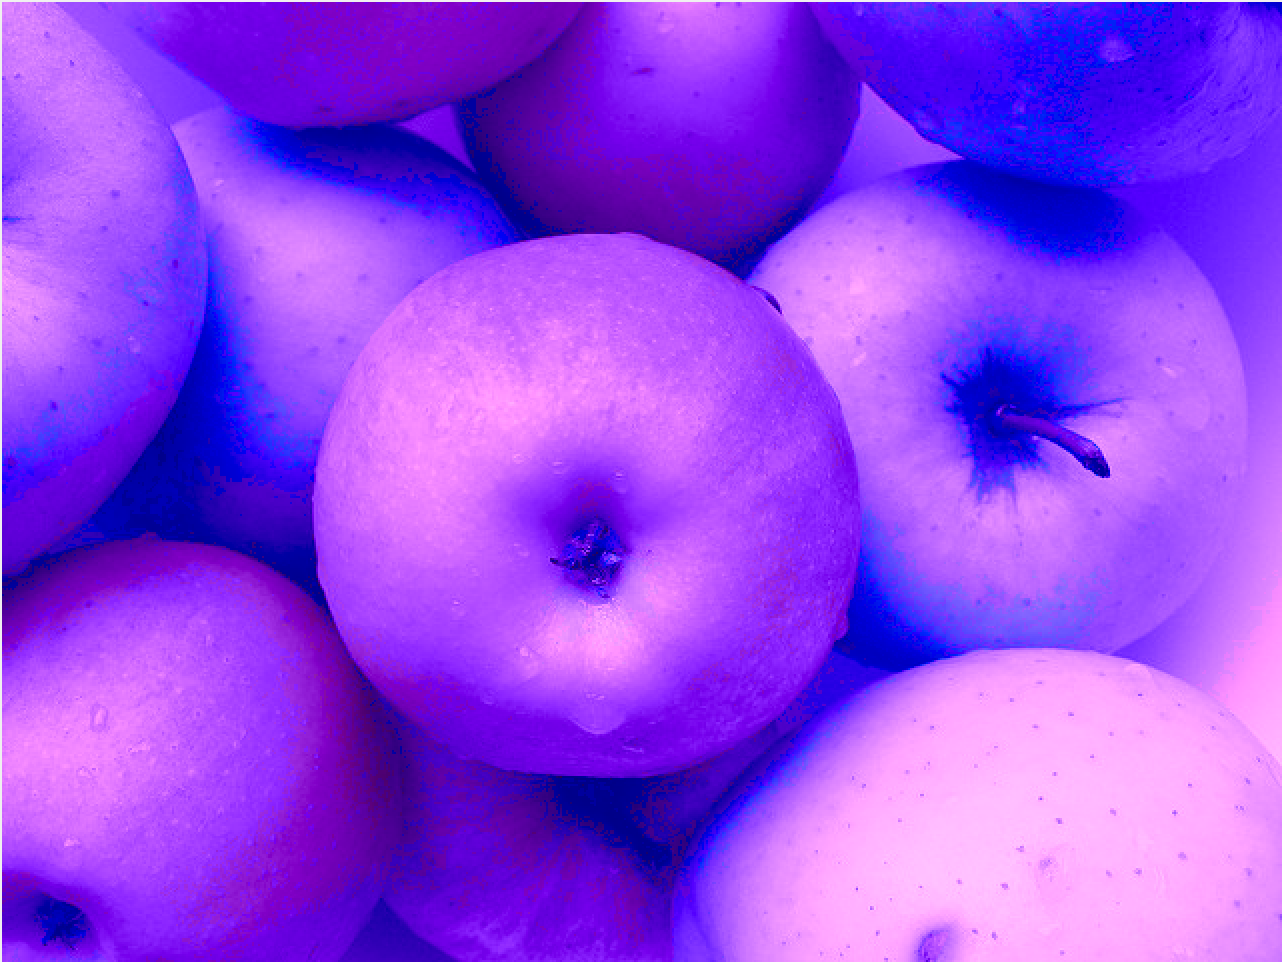
\includegraphics[width=.9\linewidth]{AnimalVision/1.png}
	\caption*{1}
\end{subfigure}%
\begin{subfigure}{.33\textwidth}
	\centering
	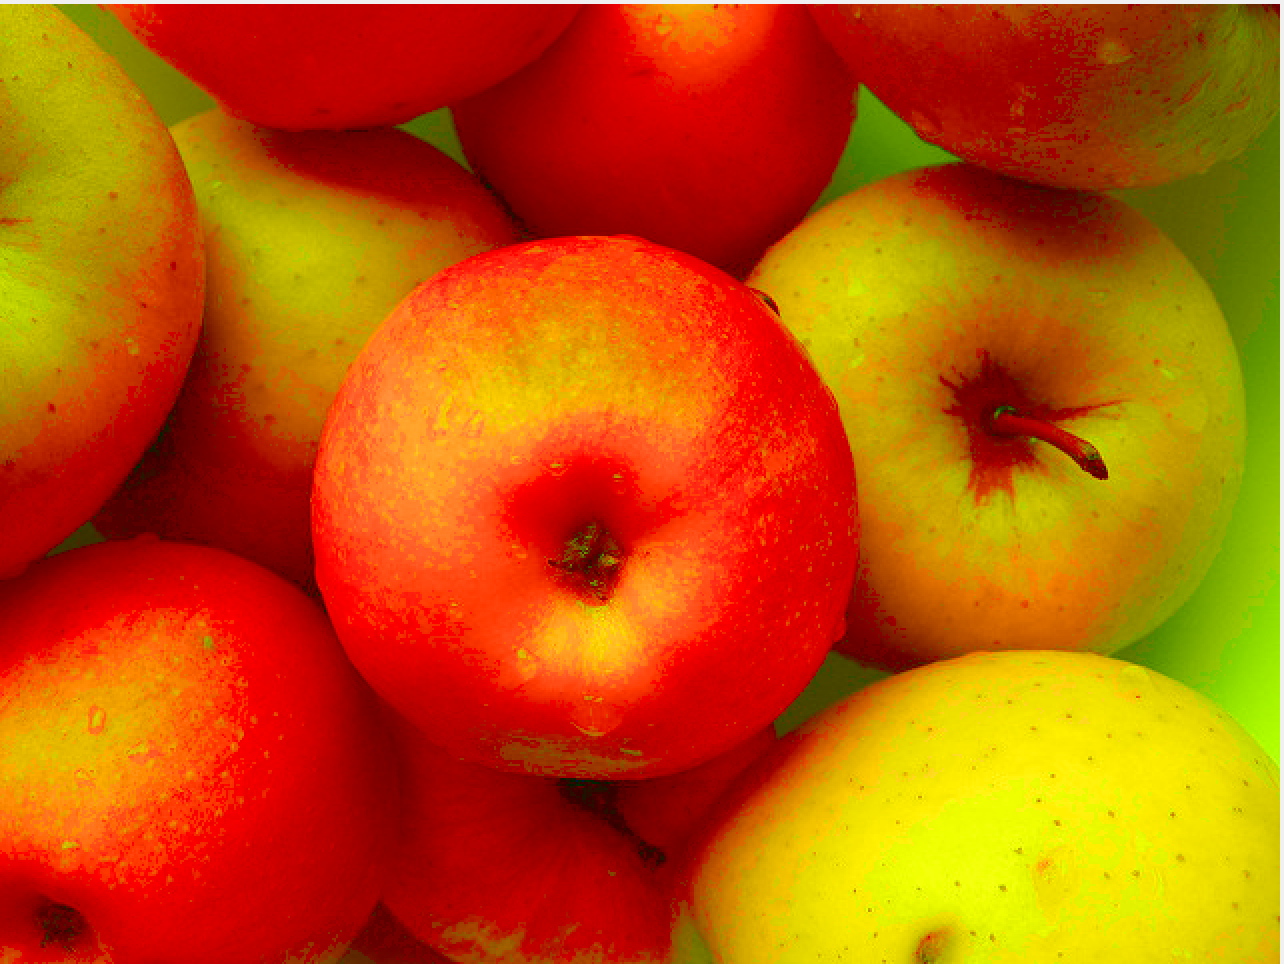
\includegraphics[width=.9\linewidth]{AnimalVision/2.png}
	\caption*{2}
\end{subfigure}%
\begin{subfigure}{.33\textwidth}
	\centering
	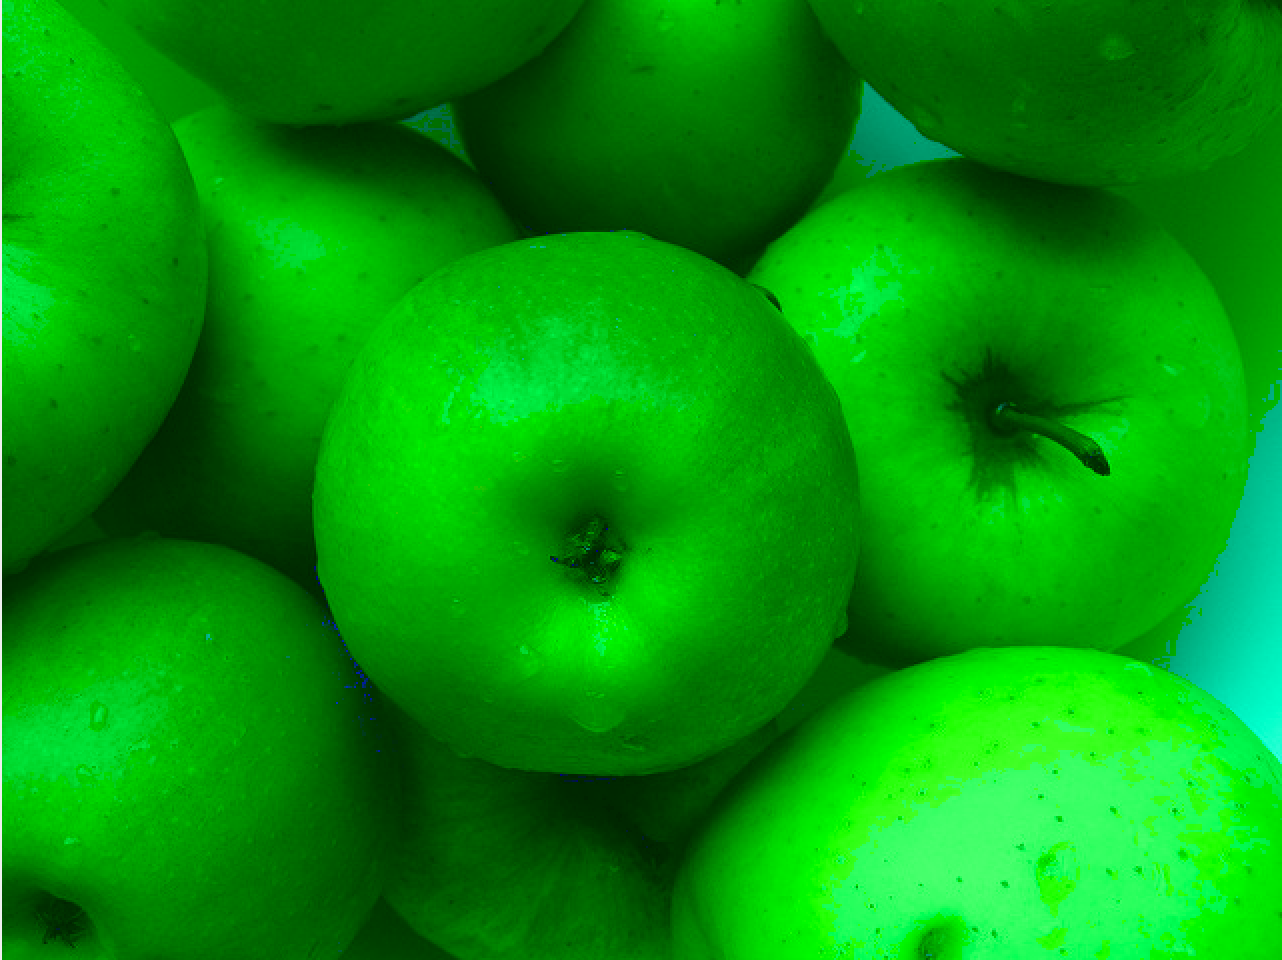
\includegraphics[width=.9\linewidth]{AnimalVision/3.png}
	\caption*{3}
\end{subfigure}
\end{figure}

For comparison, the input image is the following\footnote{Taken from Flickr user zaveqna, “Apples,” (2008). Accessed March 2017, \url{https://www.flickr.com/photos/zaveqna/2872120203/}}:

\begin{figure}[h]
	\centering
	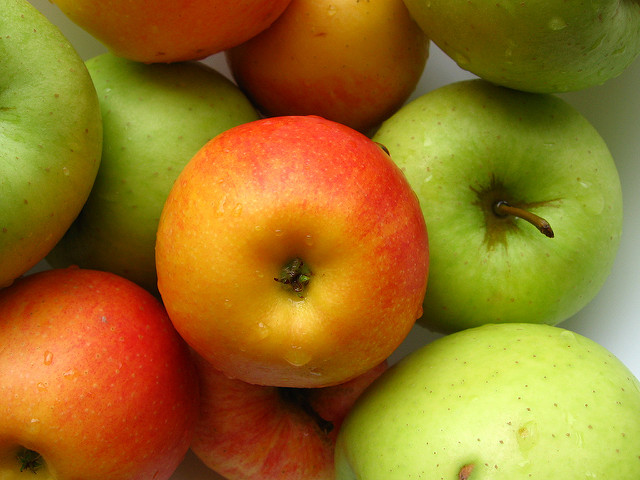
\includegraphics[width=.3\linewidth]{apples.jpg}
	\caption*{Apples.jpg}
\end{figure}


\section{Our Application}
\subsection{Basic Application (Yannick Grimault)}

For now, our application doesn't do much. We simply have a menu that can redirect the user towards one of the features which are not yet implemented. We also put an ``About us'' section that gives information to the user about this project. Because it is just a text, we can add a part explaining how the application works too, but this is not our immediate goal.

\begin{figure}[h]
\begin{subfigure}{.25\textwidth}
	\centering
	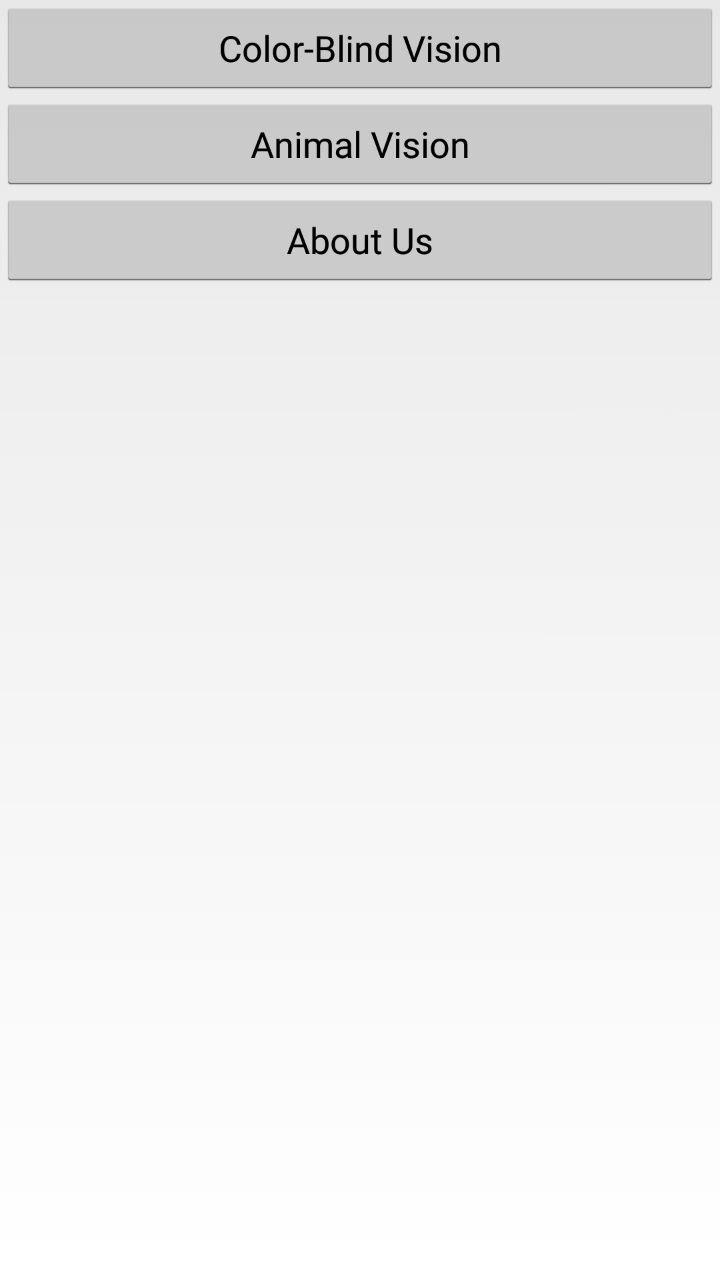
\includegraphics[width=.9\linewidth]{ApplicationScreenshots/MainMenu.jpg}
	\caption*{Main Menu}
\end{subfigure}%
\begin{subfigure}{.25\textwidth}
	\centering
	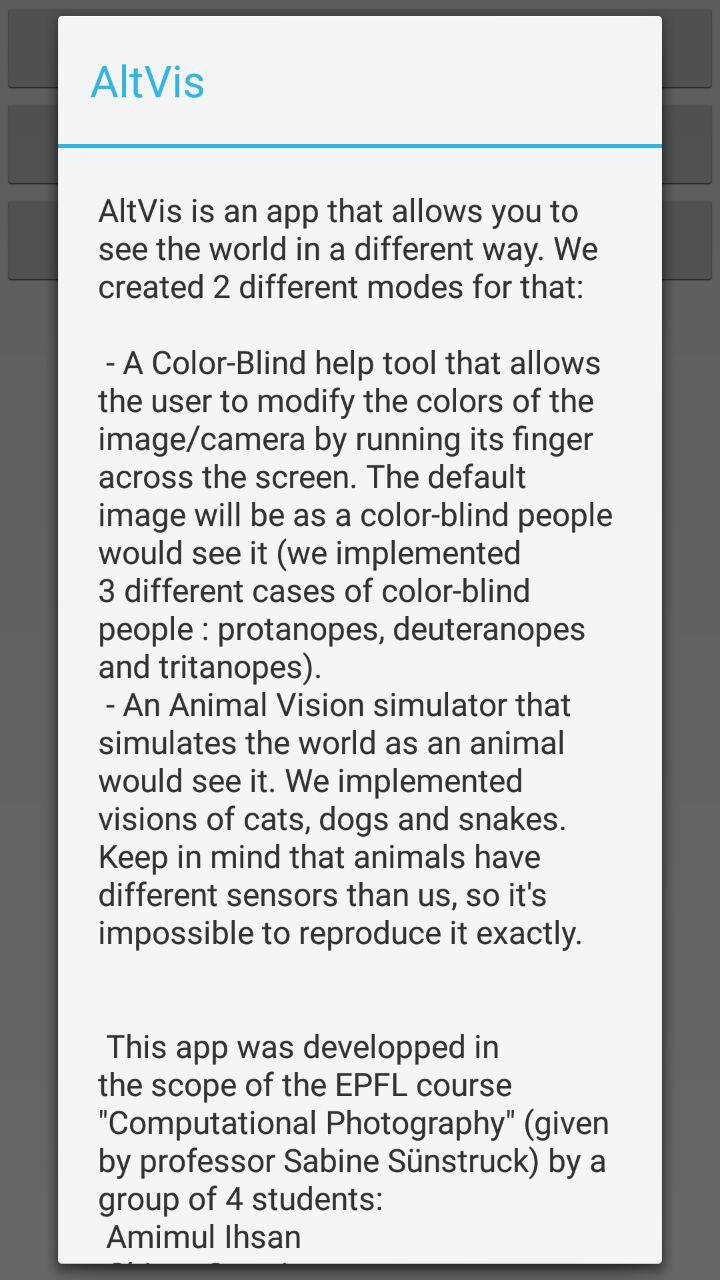
\includegraphics[width=.9\linewidth]{ApplicationScreenshots/AboutUs.jpg}
	\caption*{About Us}
\end{subfigure}%
\begin{subfigure}{.25\textwidth}
	\centering
	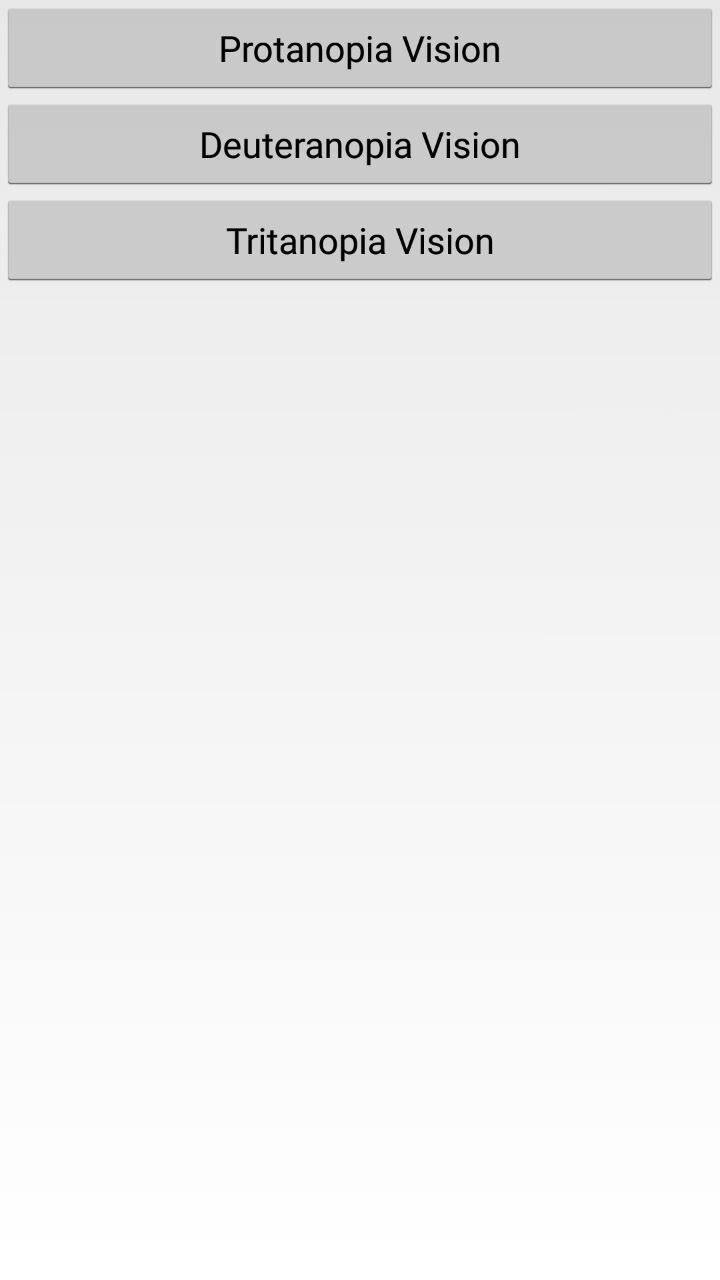
\includegraphics[width=.9\linewidth]{ApplicationScreenshots/ColorBlind.jpg}
	\caption*{Color Blind Menu}
\end{subfigure}%
\begin{subfigure}{.25\textwidth}
	\centering
	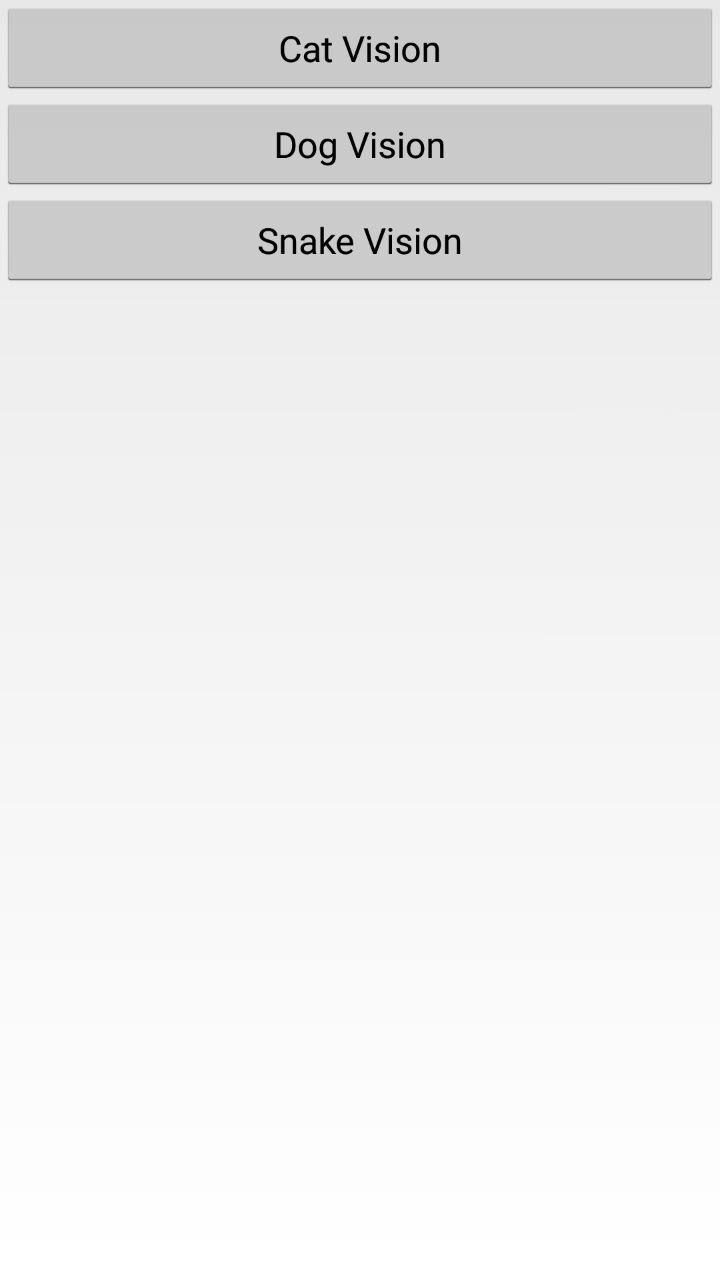
\includegraphics[width=.9\linewidth]{ApplicationScreenshots/AnimalVision.jpg}
	\caption*{Animal Vision Menu}
\end{subfigure}
\end{figure}



%%%%% Ne rien rajouter à partir d'ici

\end{document}